% Source: Wald GR, physical PDF p. 167
%         (printed p. 154).
% Coverage: Figure 6.9, the Kruskal extension of Schwarzschild spacetime.
% Figures/tables/footnotes: Figure 6.9; no tables or footnotes.
% Status: source-reviewed and compile-clean.
% Uncertainties: none.
\begingroup
\renewcommand{\thefigure}{6.9}
\begin{figure}[htbp]
\centering
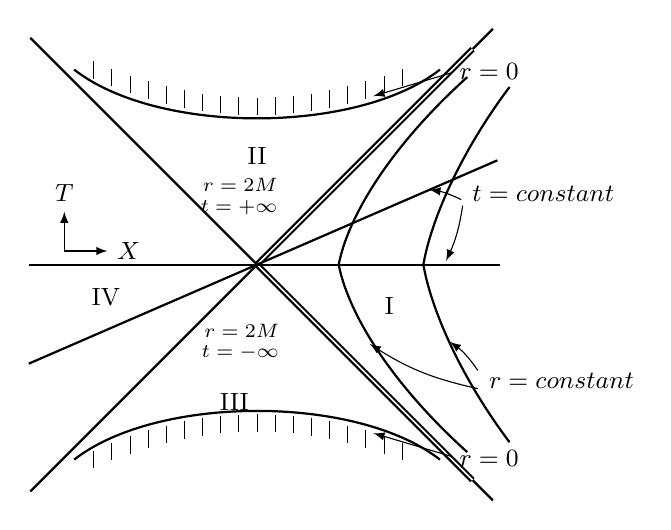
\begin{tikzpicture}[scale=.96,>=latex,font=\small]
  \draw[thick] (-3.0,-3.0) -- (3.12,3.12);
  \draw[thick] (-3.0,3.0) -- (3.12,-3.12);
  \draw[thick,double] (0,0) -- (2.85,2.85);
  \draw[thick,double] (0,0) -- (2.85,-2.85);
  \draw[thick] (2.78,-2.48)
    .. controls (1.74,-1.54) and (1.20,-.62) .. (1.08,0)
    .. controls (1.20,.62) and (1.74,1.54) .. (2.78,2.48);
  \draw[thick] (3.34,-2.35)
    .. controls (2.68,-1.47) and (2.30,-.58) .. (2.20,0)
    .. controls (2.30,.58) and (2.68,1.47) .. (3.34,2.35);
  \draw[thick] (-3.02,0) -- (3.22,0);
  \draw[thick] (-3.02,-1.31) -- (3.18,1.38);
  \draw[thick] (-2.42,2.58) .. controls (-1.32,1.72) and (1.32,1.72) .. (2.42,2.58);
  \draw[thick] (-2.42,-2.58) .. controls (-1.32,-1.72) and (1.32,-1.72) .. (2.42,-2.58);
  \foreach \x in {-2.16,-1.92,...,2.16} {
    \draw (\x,{1.98+.103*\x*\x}) -- ++(0,.23);
    \draw (\x,{-1.98-.103*\x*\x}) -- ++(0,-.23);
  }
  \node at (1.75,-.55) {I};
  \node at (0,1.44) {II};
  \node at (-.30,-1.82) {III};
  \node at (-2.00,-.43) {IV};
  \node[font=\scriptsize,left] at (.40,1.05) {\(r=2M\)};
  \node[font=\scriptsize,left] at (.40,.76) {\(t=+\infty\)};
  \node[font=\scriptsize,left] at (.42,-.88) {\(r=2M\)};
  \node[font=\scriptsize,left] at (.42,-1.17) {\(t=-\infty\)};
  \draw[->] (2.58,2.54) -- (1.54,2.23);
  \node[right] at (2.55,2.56) {\(r=0\)};
  \draw[->] (2.58,-2.54) -- (1.54,-2.23);
  \node[right] at (2.55,-2.56) {\(r=0\)};
  \node[right] at (2.94,-1.54) {\(r=\text{constant}\)};
  \draw[->] (2.92,-1.40) to[bend right=10] (2.55,-1.02);
  \draw[->] (2.92,-1.64) to[bend left=10] (1.49,-1.05);
  \node[right] at (2.72,.94) {\(t=\text{constant}\)};
  \draw[->] (2.70,.86) to[bend right=9] (2.28,.99);
  \draw[->] (2.72,.78) to[bend left=8] (2.50,.05);
  \draw[->] (-2.55,.18) -- (-2.55,.70) node[above] {\(T\)};
  \draw[->] (-2.55,.18) -- (-1.98,.18) node[right] {\(X\)};
\end{tikzpicture}
\caption{The Kruskal extension of Schwarzschild spacetime.}
\label{fig:6.9}
\end{figure}
\endgroup
